% This is the Reed College LaTeX thesis template. Most of the work
% for the document class was done by Sam Noble (SN), as well as this
% template. Later comments etc. by Ben Salzberg (BTS). Additional
% restructuring and APA support by Jess Youngberg (JY).
% Your comments and suggestions are more than welcome; please email
% them to cus@reed.edu
%
% See http://web.reed.edu/cis/help/latex.html for help. There are a
% great bunch of help pages there, with notes on
% getting started, bibtex, etc. Go there and read it if you're not
% already familiar with LaTeX.
%
% Any line that starts with a percent symbol is a comment.
% They won't show up in the document, and are useful for notes
% to yourself and explaining commands.
% Commenting also removes a line from the document;
% very handy for troubleshooting problems. -BTS

% As far as I know, this follows the requirements laid out in
% the 2002-2003 Senior Handbook. Ask a librarian to check the
% document before binding. -SN

%%
%% Preamble
%%
% \documentclass{<something>} must begin each LaTeX document
\documentclass[12pt,twoside]{reedthesis}
% Packages are extensions to the basic LaTeX functions. Whatever you
% want to typeset, there is probably a package out there for it.
% Chemistry (chemtex), screenplays, you name it.
% Check out CTAN to see: http://www.ctan.org/
%%
\usepackage{graphicx,latexsym}
\usepackage[french]{babel} 
\usepackage{amsmath}
\usepackage{amssymb,amsthm}
\usepackage[dvipsnames]{xcolor} % tk: for more color
\usepackage{xcolor}
\usepackage{eso-pic}
\usepackage{longtable,booktabs,setspace}
\usepackage{chemarr} %% Useful for one reaction arrow, useless if you're not a chem major
\usepackage[hyphens]{url}
\usepackage{tikz}
\usetikzlibrary{calc}
\newcommand\HRule{\rule{\textwidth}{1pt}}
% Added by CII
\usepackage{hyperref}
\usepackage{lmodern}
\usepackage{float}
\floatplacement{figure}{H}
% End of CII addition
\usepackage{rotating}
\usepackage{upgreek} % tk : pour pouvoir utiliser le symbole µ droit (pas en itallic)



% Next line commented out by CII
%%% \usepackage{natbib}
% Comment out the natbib line above and uncomment the following two lines to use the new
% biblatex-chicago style, for Chicago A. Also make some changes at the end where the
% bibliography is included.
%\usepackage{biblatex-chicago}
%\bibliography{thesis}


% Added by CII (Thanks, Hadley!)
% Use ref for internal links
\renewcommand{\hyperref}[2][???]{\autoref{#1}}
\def\chapterautorefname{Chapter}
\def\sectionautorefname{Section}
\def\subsectionautorefname{Subsection}
% End of CII addition

% Added by CII
\usepackage{caption}
\captionsetup{width=5in}
% End of CII addition

% \usepackage{times} % other fonts are available like times, bookman, charter, palatino


% To pass between YAML and LaTeX the dollar signs are added by CII
\title{THÈSE}
\author{Thomas Karaouzene}
\labo{}
% The month and year that you submit your FINAL draft TO THE LIBRARY (May or December)
\date{31 octobre 2017}
\division{}
\advisor{Pierre Ray}
%If you have two advisors for some reason, you can use the following
% Uncommented out by CII
\altadvisor{Nicolas Thierry-Mieg}
% End of CII addition

%%% Remember to use the correct department!
\department{Ingénierie de la Santé, de la Cognition et Environnement (EDISCE)}
% if you're writing a thesis in an interdisciplinary major,
% uncomment the line below and change the text as appropriate.
% check the Senior Handbook if unsure.
%\thedivisionof{The Established Interdisciplinary Committee for}
% if you want the approval page to say "Approved for the Committee",
% uncomment the next line
%\approvedforthe{Committee}

% Added by CII
%%% Copied from knitr
%% maxwidth is the original width if it's less than linewidth
%% otherwise use linewidth (to make sure the graphics do not exceed the margin)
\makeatletter
\def\maxwidth{ %
  \ifdim\Gin@nat@width>\linewidth
    \linewidth
  \else
    \Gin@nat@width
  \fi
}
\makeatother

\renewcommand{\contentsname}{Table of Contents}
% End of CII addition

\setlength{\parskip}{0pt}

% Added by CII
  %\setlength{\parskip}{\baselineskip}
  \usepackage[parfill]{parskip}

\providecommand{\tightlist}{%
  \setlength{\itemsep}{0pt}\setlength{\parskip}{0pt}}

\Acknowledgements{

}

\Dedication{

}

\Preface{
This is an example of a thesis setup to use the reed thesis document
class (for LaTeX) and the R bookdown package, in general.
}

\Abstract{

}

	\usepackage{tikz}
% End of CII addition
%%
%% End Preamble
%%
%

\usepackage{amsthm}
\newtheorem{theorem}{Theorem}[section]
\newtheorem{lemma}{Lemma}[section]
\theoremstyle{definition}
\newtheorem{definition}{Definition}[section]
\newtheorem{corollary}{Corollary}[section]
\newtheorem{proposition}{Proposition}[section]
\theoremstyle{definition}
\newtheorem{example}{Example}[section]
\theoremstyle{remark}
\newtheorem*{remark}{Remark}
\begin{document}

% Everything below added by CII
      \maketitle
  
  \frontmatter % this stuff will be roman-numbered
  \pagestyle{empty} % this removes page numbers from the frontmatter

  
      \begin{preface}
      This is an example of a thesis setup to use the reed thesis document
      class (for LaTeX) and the R bookdown package, in general.
    \end{preface}
  
      \hypersetup{linkcolor=black}
    \setcounter{tocdepth}{3}
    \tableofcontents
  
      \listoftables
  
      \listoffigures
  
  
  
  \mainmatter % here the regular arabic numbering starts
  \pagestyle{fancyplain} % turns page numbering back on

  \chapter{Delete line 6 if you only have one
  advisor}\label{delete-line-6-if-you-only-have-one-advisor}
  
  \chapter*{Remerciements}\label{remerciements}
  \addcontentsline{toc}{chapter}{Remerciements}
  
  \chapter*{Résumé}\label{resume}
  \addcontentsline{toc}{chapter}{Résumé}
  
  \chapter{Introduction}\label{introInf}
  
  \chapter{Investigation génétique et physiologique de la
  globozoospermie}\label{globo}
  
  \section{Introduction sur la
  globozoospermie}\label{introduction-sur-la-globozoospermie}
  
  Comme expliqué précédemment, La globozoospermie est phénotype rare
  (\textless{} 0.1\% des patients infertiles) mais néanmoins sévère (Sen,
  Holstein, \& Schirren, \protect\hyperlink{ref-Sen2009}{1971}) de
  teratozoospermie menant à l'infertilité masculine. Cette anomalie est
  caractérisée par la présence de spermatozoïdes présentant une tête ronde
  dépourvue d'acrosome et d'une pièce intermédiaire désorganisée dans
  l'éjaculat (Singh, n.d., Pedersen \& Rebbe
  (\protect\hyperlink{ref-Pedersen1974}{1974})) (\textbf{Figure :
  }\ref{fig:globospz}). En plus des anomalies morphologiques, les
  spermatozoïdes globozoocéphales présentent également des
  désorganisations au niveau moléculaire. Par exemple, le facteur
  spermatique PLC\(\zeta\) requit pour l'activation ovocitaire, est absent
  ou en quantité infime dans les spermatozoïdes globozoocéphales (Heytens
  et al., \protect\hyperlink{ref-Heytens2009}{2009}, Taylor et al.
  (\protect\hyperlink{ref-Taylor2010}{2010}), S.-Y. Yoon et al.
  (\protect\hyperlink{ref-Yoon2008}{2008})) compromettant ainsi
  l'activation ovocytaire et expliquant le faible taux de fécondation
  observés en IVF (\emph{in vitro} fertilization) et en ICSI (intra
  cytoplasmic sperm injection) (A. Dam et al.,
  \protect\hyperlink{ref-Dam2006}{2006}). On distingue la globozoospermie
  totale avec 100\% des spermatozoïdes présentant le phénotype ou
  partielle en fonction du taux de spermatozoïdes atteints. Bien que
  l'infertilité masculine soit souvent la résultante de plusieurs
  facteurs, les premières études présentant des patients atteints par un
  phénotype complet (Sen et al., \protect\hyperlink{ref-Sen2009}{1971})
  suggéraient que la globozoospermie était une exception. De plus les
  caractéristiques morphologiques très typiques des spermatozoïdes
  laissaient penser à une cause monogénique. En 2007, une étude portant
  sur une famille juive ashkénaze comprenant six frères dont trois atteins
  a pu lier ce phénotype à une mutation homozygotes sur le gène
  \emph{SPATA16} présente chez les trois frères atteint (A. H. D. M. Dam
  et al., \protect\hyperlink{ref-Dam2007}{2007}). Cependant, dans la même
  étude, 29 autres patients présentant le même phénotype ont été analysé,
  et pour ceux-ci, aucun variant du gène \emph{SPATA16} n'a pu être lié au
  phénotype (A. H. D. M. Dam et al.,
  \protect\hyperlink{ref-Dam2007}{2007}) indiquant clairement que les
  mutations de ce gène n'étaient pas les seules responsables. En 2011, une
  autre étude portant sur une cohorte de 20 patients Tunisiens a pu mettre
  en évidence une délétion homozygote de 200kb emportant la totalité du
  gène \emph{DPY19L2} chez 15 des 20 patients analysés (Harbuz et al.,
  \protect\hyperlink{ref-Harbuz2011}{2011}). Les études effectuées
  ultérieurement sur ce phénotype ont ensuite pu montrer que les
  altérations du gène \emph{DPY19L2}, et notamment cette délétion, étaient
  responsables de la majorité des cas de globozoospermie (P. F. Ray \&
  Arnoult, \protect\hyperlink{ref-Ray2011}{2011}, ElInati et al.
  (\protect\hyperlink{ref-ElInati2012}{2012})).
  
  \begin{figure}
  
  {\centering 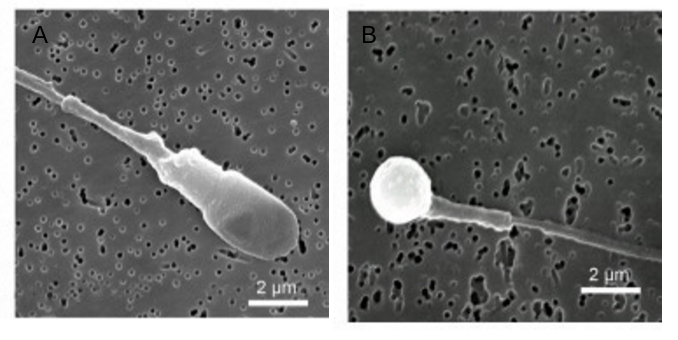
\includegraphics[scale=0.50]{figure/globo_normal_spz} 
  
  }
  
  \caption[Observation au microscope à balayage d'un spermatozoïde normal (**A**) et d'un spermatozoïde globozoocéphale (**B**) (changer les photos avec celles sur lesquelles on voit l'acrosome colorés)]{Observation au microscope à balayage d'un spermatozoïde normal (**A**) et d'un spermatozoïde globozoocéphale (**B**) (changer les photos avec celles sur lesquelles on voit l'acrosome colorés) adapté d'après [@Harbuz2011]}\label{fig:globospz}
  \end{figure}
  
  En 2012, le développement d'un modèle murin KO \emph{Dpy19l2}\(^{-/-}\)
  a permis de mieux comprendre les mécanismes moléculaires impliqué dans
  la globozoospermie causée par la délétion du gène \emph{DPY19L2} chez
  l'humain (V. Pierre et al., \protect\hyperlink{ref-Pierre2012}{2012}).
  Tout d'abord car ce modèle de souris KO présentait les mêmes
  caractéristiques que les patients humains. Tout d'abord, ces souris
  étaient infertiles et présentaient des spermatozoïdes globozoocéphales
  (\textbf{Figure : }\ref{fig:mouseglobo}) mais aussi et surtout,
  l'ensembles des autres dysfonctionnements étaient retrouvés, c'est à
  dire : l'absence de l'acrosome, les défauts morphologiques du noyau, de
  l'enveloppe nucléaire et de l'acroplaxome ainsi que le mauvais
  positionnement de la manchette (V. Pierre et al.,
  \protect\hyperlink{ref-Pierre2012}{2012}). Ainsi il a pu être démontré
  que la protéine Dpy19l2 étaient principalement exprimé dans le
  spermatides et plus spécifiquement dans la membrane nucléaire interne
  faisant face à la vésicule acrosomale et que l'absence de cette protéine
  entrainait la déstabilisation à la fois de la lamine nucléaire, de la
  jonction entre l'acroplaxome et l'enveloppe nucléaire (V. Pierre et al.,
  \protect\hyperlink{ref-Pierre2012}{2012}).
  
  \begin{figure}
  
  {\centering 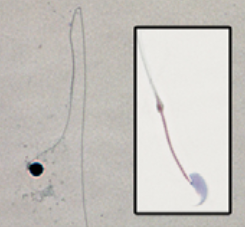
\includegraphics[scale=0.8]{figure/mouse_globo_spz} 
  
  }
  
  \caption[Comparaison entre les spermatozoïdes des souris *Dpy19l2*$^{-/-}$ (à gauche) et les souris sauvages *Dpy19l2*$^{+/+}$ (à droite)]{Comparaison entre les spermatozoïdes des souris *Dpy19l2*$^{-/-}$ (à gauche) et les souris sauvages *Dpy19l2*$^{+/+}$ (à droite) d'après [@Pierre2012]}\label{fig:mouseglobo}
  \end{figure}
  
  Dans ce chapitre je détaillerai les résultats de trois articles dont je
  suis co-auteur :
  
  \begin{enumerate}
  \def\labelenumi{\arabic{enumi}.}
  \tightlist
  \item
    \protect\hyperlink{mecamut}{\textbf{Fine Characterisation of a
    Recombination Hotspot at the DPY19L2 Locus and Resolution of the
    Paradoxical Excess of Duplications over Deletions in the General
    Population}} : au cours de cette étude j'ai participé à divers
    manipulation de biologie moléculaire tel que l'extraction d'ADN
    spermatique, quantification des délétions / duplications \emph{de
    novo}. De même, j'ai pu contribuer au divers analyses statistiques.\\
  \item
    \protect\hyperlink{transcriptome}{\textbf{Comparative testicular
    transcriptome of wild type and globozoospermic Dpy19l2 knock out
    mice}} : Dans cette étude j'ai pu effectuer l'intégralité des
    manipulation de biomoléculaire (extraction de l'ARN testiculaire de
    souris et analyse sur puce) de même que l'intégralité de l'analyse
    bioinformatique des résultats.
  \end{enumerate}
  
  \newpage
  
  \section{Résultats}\label{resultats}
  
  \hypertarget{mecamut}{\subsection{Les mécanismes
  mutationnels}\label{mecamut}}
  
  \subsubsection{Confirmation de l'excès de
  délétion}\label{confirmation-de-lexces-de-deletion}
  
  Chez les mammifères il existe trois paralogues de \emph{DPY19L2} de
  fonction encore inconnue et un pseudogène présentant une très forte
  homologie de séquence (\textgreater{} 95\%) (Carson, Cheung, \& Scherer,
  \protect\hyperlink{ref-Carson2006}{2006}). Chez l'Homme, ce gène est
  flanqué de deux séquences présentant une forte homologie
  (\textgreater{}95\%) d'une taille de 28kb (\textbf{Figure :
  }\ref{fig:nahr} - \textbf{1}). Ces séquences appelées LCRs (\emph{low
  copy repeats}) représentent une large portion du génome humain (Cheung
  et al., \protect\hyperlink{ref-Cheung2003}{2003}, Bailey et al.
  (\protect\hyperlink{ref-Bailey2002}{2002})) et vont, de par leur
  homologie favoriser les duplications de gènes jouant ainsi un rôle
  important dans l'évolution des génomes des vertébrés (Walsh,
  \protect\hyperlink{ref-Walsh2003}{2003}, Ohno
  (\protect\hyperlink{ref-Ohno1970}{1970})). Dans le cas de
  \emph{DPY19L2}, ces LCRs vont, au cours de la méiose entrainer la venue
  de recombinaison homologues non-allélique (NAHR) donnant lieu soit à une
  délétion du gène \emph{DPY19L2} et la formation d'un ADN circulaire
  comprenant le gène (\textbf{Figure : }\ref{fig:nahr} - \textbf{2}) soit
  à un allèle possédant deux copies du gène tandis que l'autre n'en
  possède aucune (\textbf{Figure : }\ref{fig:nahr} - \textbf{3}).
  
  Ainsi, le mécanisme de NAHR devrait, en théorie, engendrer la formation
  de plus d'allèle délété que d'allèle dupliqué puisque les cas présentés
  en figures \ref{fig:nahr} - \textbf{2} et \ref{fig:nahr} - \textbf{3}
  induisent la formation d'un allèle délété tandis que seul le cas
  \ref{fig:nahr} - \textbf{3} forme un allèle dupliqué. Cependant, les
  données mises à disposition par la base de donnée
  \href{http://dgv.tcag.ca/dgv/app/home}{\emph{Database of Genomic
  Variants}} (MacDonald, Ziman, Yuen, Feuk, \& Scherer,
  \protect\hyperlink{ref-MacDonald2014}{2014}) indique un excès de
  duplication puisque sur un total de 6575 individus analysés, un totlal
  de 83 duplications et de 26 délétions hétérozygotes ont été observées
  pour le locus de \emph{DPY19L2}. Afin de confirmer ces résultats et
  ainsi écarter l'hypothèse d'un biais causé par la présence du pseudogène
  \emph{DPY19L2P1} très homologue avec \emph{DPY19L2} (Carson et al.,
  \protect\hyperlink{ref-Carson2006}{2006}) notre équipe a procedé à
  l'analyse du locus de \emph{DPY19L2} de 1699 individus par CGHarray. Un
  total de 15 duplication et de 3 délétions hétérozygotes furent observés
  
  \begin{figure}
  
  {\centering 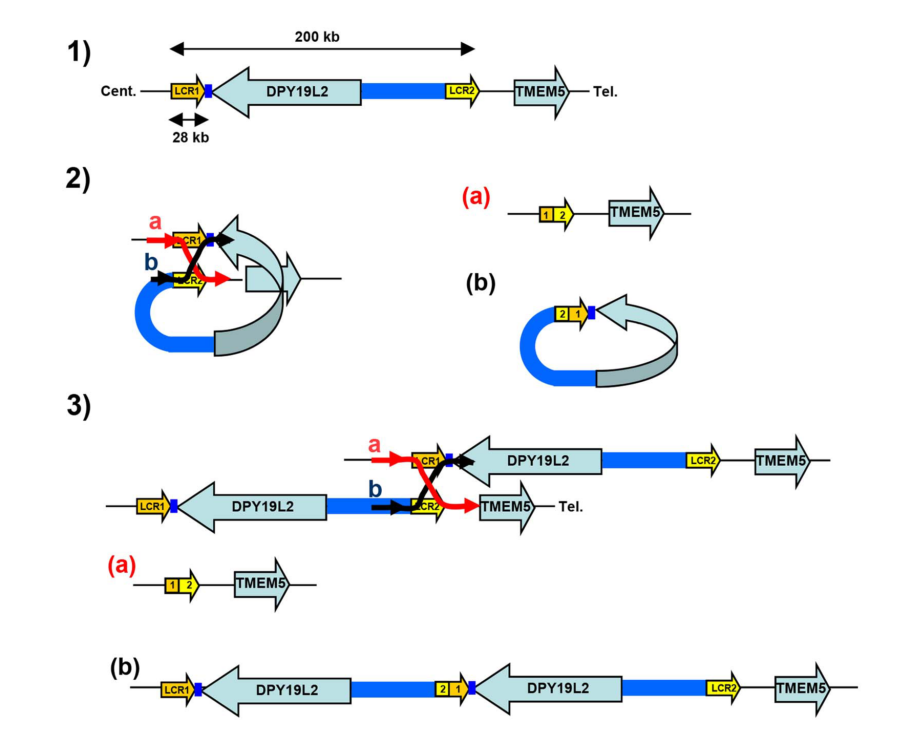
\includegraphics[scale=0.5]{figure/dpy_nahr} 
  
  }
  
  \caption[Représentation schématique du mécanisme de NAHR causé par les séquences LCR flanquant le gène *DPY19L2*]{Représentation schématique du mécanisme de NAHR causé par les séquences LCR flanquant le gène *DPY19L2* : **1** : Le gène *DPY19L2* est entouré par les séquences LCR1 et LCR2 qui correspondent respectivement au LCR centromérique et télomérique. Ces LCRs sont séparés par environs 200kb et chacun d'eux mesurent approximativement 28kb. **2** : NAHR résultant du mauvais alignement des LCRs 1 et 2 du même chromatide entrainant la formation d'un allèle délété (a) et d'un ADN circulaire comprenant le gène *DPY19L2*. Cet ADN circulaire sera éliminé au cours du cycle cellulaire. **3** : NAHR résultant du mauvais alignement des LCRs 1 et 2 provenant de deux chromatides différents conduisant à la formation d'un allèle délété (a) et d'un allèle dupliqué (b)}\label{fig:nahr}
  \end{figure}
  
  \subsubsection{\texorpdfstring{Détermination du taux de recombinaison
  \emph{de novo} de
  \emph{DPY19L2}}{Détermination du taux de recombinaison de novo de DPY19L2}}\label{determination-du-taux-de-recombinaison-de-novo-de-dpy19l2}
  
  Alors que les résultats précédents confirment un excès de l'allèle
  dupliqué de \emph{DPY19L2} dans la population générale, nous avons par
  la suite cherché à déterminer les fréquences de duplications / délétions
  \emph{de novo} de ce même locus. Ceci ayant pour but de déterminer si
  cet exces est dû à une séléction de l'allèle dupliqué ou au fait que
  celui-ci était effectivement produit plus fréquement que l'allèle
  délété. Pour ce faire nous avons quantifié le taux d'apparition de ces
  événements génétiques à partir d'ADN spermatique. Les spermatozoïdes
  étant le produits direct de la méiose, ils sont donc les reflets
  d'haplotypes produits \emph{de novo}. Pour cela, nous avons analyser par
  PCR digitale l'ADN spermatique de trois donneurs. Leur ADN a tout d'abor
  été dilué en série de sorte à ce qu'environ 25\% des 96 puits de la PCR
  contiennent un événement (délétion ou duplication). Ainsi, en acceptant
  qu'un génome haploïde humain représente 3pg, 50ng d'ADN spermatique
  furent déposés dans chaque puit pour la PCR spécifique à la délétion, et
  100ng dans chaque puit spécifiques à a duplication. Chaque puit contient
  donc une partie de cette charge d'ADN initiale. La distribution de cette
  charge d'ADN au sein des 96 puits peut donc s'apparier à un tirage sans
  remise, la probabilité qu'un puit soit positif pour un événement
  chromosomique (duplication ou délétion) peut donc être modélisé par une
  loi hypergéométrique (\textbf{Équation} : \eqref{eq:hypergeo}). Nous
  permettant ainsi d'estimer la fréquence duplication / délétion
  \(\lambda\) pour chaque donneur (\textbf{Équation} : \eqref{eq:lambda})
  (\textbf{Figure : }\ref{fig:dupdelrate}).
  
  \begin{equation} 
  \frac{\frac{(N - R)!}{W!(N-R-W)!}}{\frac{N!}{W!(N-W)!}} = \frac{(N-R)!(N-W)!}{N!(N-W-R)!} = \prod_{i=0}^{R-1}{\frac{N-W-i}{N-i}}
  \label{eq:hypergeo}
  \end{equation}
  
  \begin{equation} 
  \lambda = \frac{R}{N}
  \label{eq:lambda}
  \end{equation}
  
  Où :\\
  . \(N\) : représente le nombre de copie de chromosome 12 dans la charge
  d'ADN initiale (1.6x10\({^6}\) pour la PCR spécifique à la délétion,
  3.2x10\({^6}\) pour la PCR spécifique à la duplication)\\
  . \(W = \frac{N}{96}\) correspond au nombre de copiede chromosome 12 par
  puit\\
  . \(R\) représente le nombre total de recombinaison observées
  
  L'interval de confiance (IC) à 95\% est ensuite calculé grâce à une loi
  binomiale de sorte à modéliser la dilution initiale pour obtenir l'ADN
  d'\emph{entrée}. Le puit contenant le \emph{pool} des trois ADN
  spermatique est donc celui ayant les résultats les plus robustes, l'IC
  étant le plus resséré (\textbf{Figure : }\ref{fig:dupdelrate}), et
  permet donc d'établir le taux de délétion \emph{de novo} à 1.8 x
  10\(^{-5}\) (IC 95\% : 1.4x 10\(^{-6}\); 2.2x 10\(^{-6}\)) tandis que le
  taux de duplication \emph{de novo} est estimé à 7.7 x 10\(^{-6}\) (IC
  95\% : 6.1 x 10\(^{-6}\); 9.7 x 10\(^{-6}\)) montrant un enrichisement
  environ deux fois supperieur des délétion par rapport aux duplications
  sur le site de \emph{DPY19L2} (\textbf{Figure : }\ref{fig:dupdelrate}).
  
  \begin{figure}
  
  {\centering 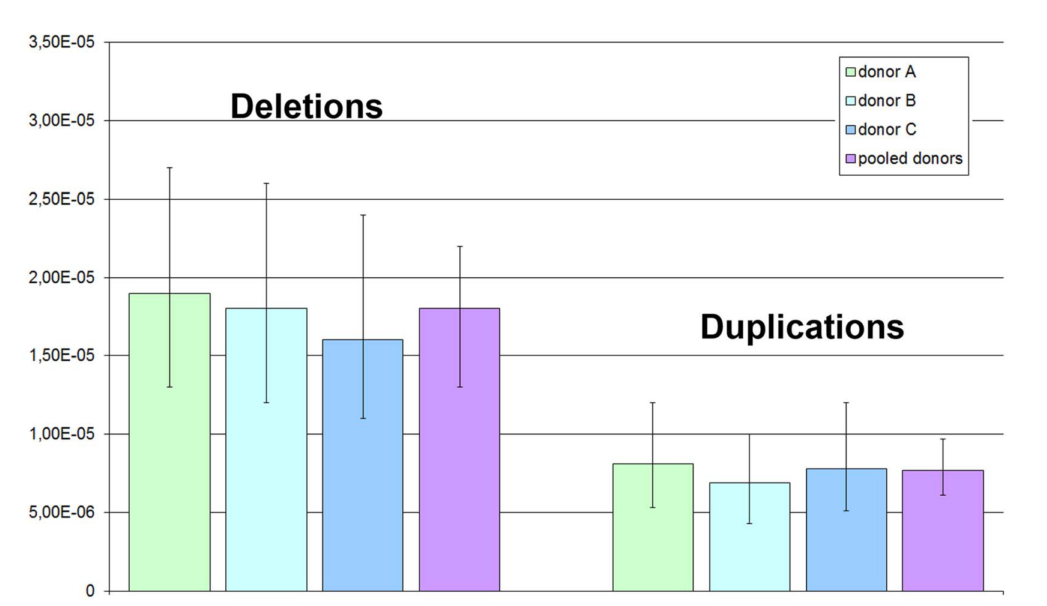
\includegraphics[scale=0.38]{figure/globo_du_del_rate} 
  
  }
  
  \caption[Ratio des délétions / duplications *de novo* observées au locus *DPY19L2* déterminé par PCR digital à partir d'ADN spermatique de trois donneurs]{Ratio des délétions / duplications *de novo* observées au locus *DPY19L2* déterminé par PCR digital à partir d'ADN spermatique de trois donneurs : [TODO]}\label{fig:dupdelrate}
  \end{figure}
  
  \subsubsection{Autres résultats}\label{autres-resultats}
  
  Cette étude a également été pour notre équipe l'occasion d'effectuer une
  étude plus approfondie des LCRs flanquant le locus de \emph{DPY19L2}.
  Ainsi, nous avons pu mettre en évidence que les LCRs 1 et 2 contenaient
  5 répétitions du site de reconnaissance consensus de PRDM9
  (CCNCCNTNNCCNC), une protéine connue pour {[}TODO : décrire le rôle de
  PRDM9{]}. De même, nous avons pu mettre en évidence que les
  recombinaisons s'effectuaient le long de 5 points de cassures distincts
  répartis le long des LCRs 1 et 2 et que comme attendu, l'incidence des
  points de cassures dans les recombinaisons du locus \emph{DPY19L2} était
  proportionelle à la taille des régions {[}TODO : expliquer mieux{]}.
  
  \hypertarget{transcriptome}{\subsection{La
  transcriptomique}\label{transcriptome}}
  
  \begin{flushleft} 
  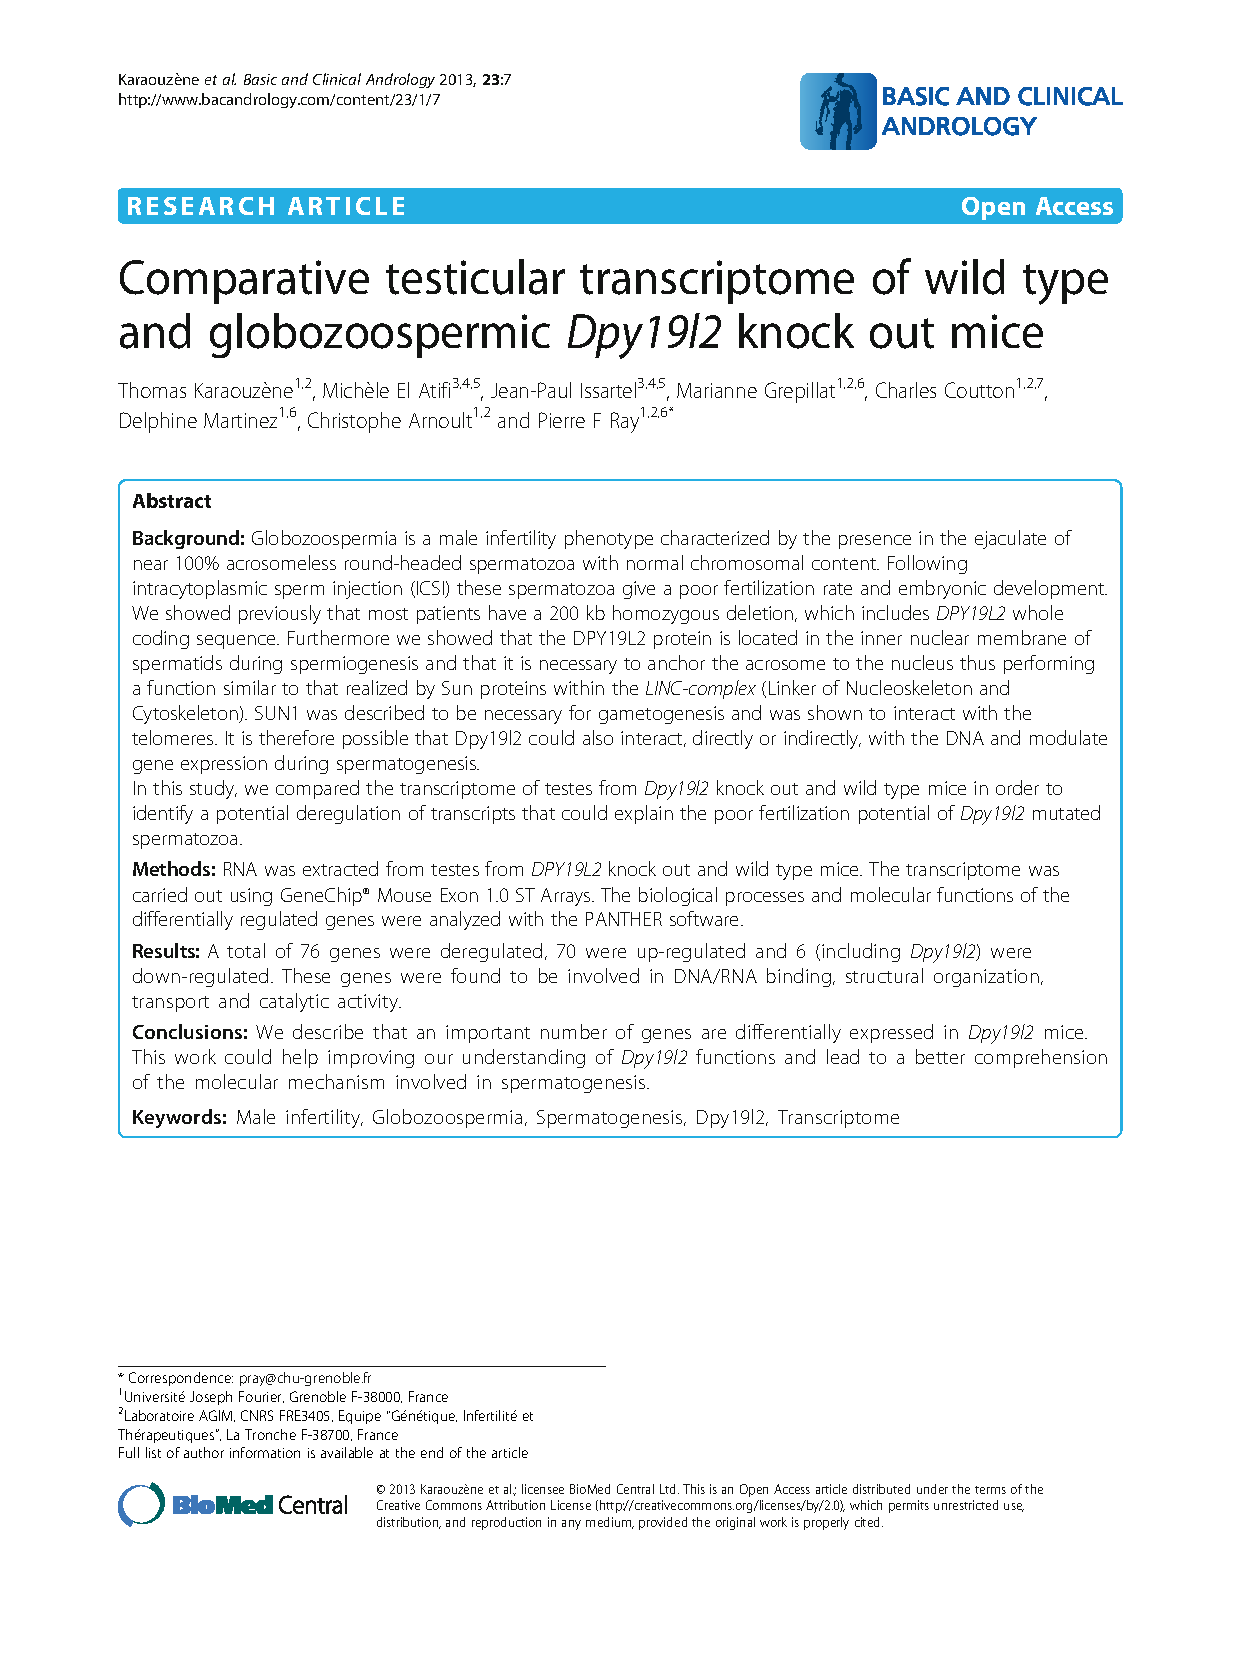
\includegraphics[width=7.5in]{/home/karaout/MaThese/index/bib/12610_2013_Article_8.pdf}
  \newpage
  \end{flushleft}
  
  Dans des études précédentes, notre équipe à réussit à démontrer que la
  protéine \emph{DPY19L2} était localisée dans la membrane interne des
  noyaux des spermatides pendant la spermatogénèse et qu'elle est
  nécessaire pour fixer l'acrosome au noyau {[}TODO: insert ref{]}. De
  même, nous avons pu mettre en évidence que dans des cellules HEK cette
  protéine colocalisait avec la protéine SUN5 et que \emph{Dpy19l2}
  pourrait être un partenaire de SUN5(V. Pierre et al.,
  \protect\hyperlink{ref-Pierre2012}{2012}). nous avons cherché à observer
  si, comme la protéine SUN5. Chez la souris, la protéine Sun1 est elle
  aussi nécéssaire à la gamétogénèse et est connue pour permettre
  l'intéraction entre le noyau et les télomères (Ding et al.,
  \protect\hyperlink{ref-Ding2007}{2007}). Dans cette étude nous avons
  donc chercher à savoir si l'absence de la protéine Dpy19l2 pouvait
  entrainer des dérèglement transcriptionelle qui pourrait, entre autre,
  expliquer l'absence de la protéine PLC\(\zeta\) dans les spermatozoïdes
  globozoocéphales.\\
  Pour cela, nous avons effectué une analyse comparative du transcriptome
  testiculaire de deux souris \emph{Dpy19l2}\(^{+/+}\) (S1+ et S2+) et
  deux souris \emph{Dpy19l2}\(^{-/-}\) (S1- et S2-). Cette analyse a été
  effectué sur des puces à ADN du type Affymetrix GeneChip® Mouse Exon 1.0
  contenant des sondes pour 35.557 gènes murins. Pour chacun de ces gènes,
  nous avons donc chercher à soivoir s'ils étaient différentiellement
  exprimés chez les sours S1- et S2- lorsqu'on comparait leur expression
  avec celle des souris S1+ et S2+ en calculant quatre ratio (R1, R2, R3
  et R4) (\textbf{Équation} : \eqref{eq:micerate}). Les gènes pour lesquels
  au moins 3 de leurs ratio étaient \(\ge\) 1,7 furent considérés comme
  sur-exprimés tandis que ceux pour lesquels 3 de leurs ratio étaient
  \(\le\) 0,58 (\(\frac{1}{1,7}\)) furent considérés comme sous-exprimés.
  
  \begin{equation} 
  \begin{split}
  \forall gene \in & \ \{genes\ in\ array\}: \\
  \\
  & R1_{gene} = \frac{exp_{gene}(S1-)}{exp_{gene}(S1+)} \ \ \ \ R2_{gene} = \frac{exp_{gene}(S2-)}{exp_{gene}(S1+)} \\
  & R3_{gene} = \frac{exp_{gene}(S1-)}{exp_{gene}(S2+)} \ \ \ \ R4_{gene} = \frac{exp_{gene}(S2-)}{exp_{gene}(S2+)} 
  \label{eq:micerate}
  \end{split}
  \end{equation}
  
  Ainsi cette étude a pu mettre en évidence la sous-expression de 6 gènes
  (incluant \emph{Dpy19l2}) et la sur-expression de 70 gènes chez les
  souris \emph{Dpy19l2}\(^{-/-}\). Parmi ces gènes, nous ne figurait pas
  Plc\(\zeta\) indiquant que l'absence de cette protéine chez les
  spermatozoïdes globozoocéphales n'étaient pas directement dûe à un
  dysfonctionnement transcriptionel. Afin de prédire les fonction
  moléculaire dans lesquels étaient impliqués ces gènes, nous nous sommes
  servi du logiciel PANTHER (Mi et al.,
  \protect\hyperlink{ref-Mi2017}{2017}). Ainsi, nous avons pu constater
  que 23 gènes codant pour des protéines de liaison étaient dérégulés,
  dont 12 sont des protéines de liaison aux acides nucléiques
  (\textbf{Figure : }\ref{fig:molfunc} - \textbf{A})
  
  plusieurs fonction moléculaire se retrouvaient enrichit dans cette liste
  de gène .
  
  \begin{figure}
  
  {\centering 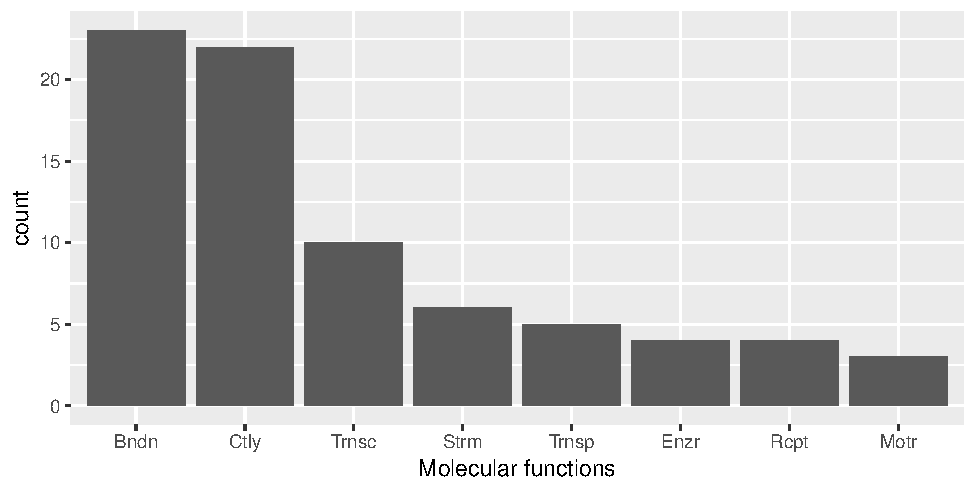
\includegraphics{thesis_files/figure-latex/molfunc-1} 
  
  }
  
  \end{figure}
  
  \section{Conclusion}\label{conclusion}
  
  \chapter{Mise en place d'une stratégie pour l'analyse des données
  exomiques -- application en recherche
  clinique}\label{mise-en-place-dune-strategie-pour-lanalyse-des-donnees-exomiques-application-en-recherche-clinique}
  
  \chapter{MutaScript}\label{mutascript}
  
  \chapter*{Conclusion}\label{conclusion-1}
  \addcontentsline{toc}{chapter}{Conclusion}
  
  \chapter{The First Appendix}\label{the-first-appendix}
  
  \chapter*{References}\label{references}
  \addcontentsline{toc}{chapter}{References}
  
  \hypertarget{refs}{}
  \hypertarget{ref-Bailey2002}{}
  Bailey, J. A., Gu, Z., Clark, R. A., Reinert, K., Samonte, R. V.,
  Schwartz, S., \ldots{} Eichler, E. E. (2002). Recent Segmental
  Duplications in the Human Genome. \emph{Science}, \emph{297}(5583),
  1003--1007. \url{http://doi.org/10.1126/science.1072047}
  
  \hypertarget{ref-Carson2006}{}
  Carson, A. R., Cheung, J., \& Scherer, S. W. (2006). Duplication and
  relocation of the functional DPY19L2 gene within low copy repeats.
  \emph{BMC Genomics}, \emph{7}, 45.
  \url{http://doi.org/10.1186/1471-2164-7-45}
  
  \hypertarget{ref-Cheung2003}{}
  Cheung, J., Estivill, X., Khaja, R., MacDonald, J. R., Lau, K., Tsui,
  L.-C., \& Scherer, S. W. (2003). Genome-wide detection of segmental
  duplications and potential assembly errors in the human genome sequence.
  \emph{Genome Biology}, \emph{4}(4), R25.
  \url{http://doi.org/10.1186/gb-2003-4-4-r25}
  
  \hypertarget{ref-Dam2007}{}
  Dam, A. H. D. M., Koscinski, I., Kremer, J. A. M., Moutou, C., Jaeger,
  A.-S., Oudakker, A. R., \ldots{} Viville, S. (2007). Homozygous mutation
  in SPATA16 is associated with male infertility in human globozoospermia.
  \emph{American Journal of Human Genetics}, \emph{81}(4), 813--20.
  \url{http://doi.org/10.1086/521314}
  
  \hypertarget{ref-Dam2006}{}
  Dam, A., Feenstra, I., Westphal, J., Ramos, L., Golde, R. van, \&
  Kremer, J. (2006). Globozoospermia revisited. \emph{Human Reproduction
  Update}, \emph{13}(1), 63--75.
  \url{http://doi.org/10.1093/humupd/dml047}
  
  \hypertarget{ref-Ding2007}{}
  Ding, X., Xu, R., Yu, J., Xu, T., Zhuang, Y., \& Han, M. (2007). SUN1 Is
  Required for Telomere Attachment to Nuclear Envelope and Gametogenesis
  in Mice. \emph{Developmental Cell}, \emph{12}(6), 863--872.
  \url{http://doi.org/10.1016/j.devcel.2007.03.018}
  
  \hypertarget{ref-ElInati2012}{}
  ElInati, E., Kuentz, P., Redin, C., Jaber, S., Vanden Meerschaut, F.,
  Makarian, J., \ldots{} Viville, S. (2012). Globozoospermia is mainly due
  to DPY19L2 deletion via non-allelic homologous recombination involving
  two recombination hotspots. \emph{Human Molecular Genetics},
  \emph{21}(16), 3695--3702. \url{http://doi.org/10.1093/hmg/dds200}
  
  \hypertarget{ref-Harbuz2011}{}
  Harbuz, R., Zouari, R., Pierre, V., Ben Khelifa, M., Kharouf, M.,
  Coutton, C., \ldots{} Ray, P. F. (2011). A recurrent deletion of DPY19L2
  causes infertility in man by blocking sperm head elongation and acrosome
  formation. \emph{American Journal of Human Genetics}, \emph{88}(3),
  351--61. \url{http://doi.org/10.1016/j.ajhg.2011.02.007}
  
  \hypertarget{ref-Heytens2009}{}
  Heytens, E., Parrington, J., Coward, K., Young, C., Lambrecht, S., Yoon,
  S.-Y., \ldots{} De Sutter, P. (2009). Reduced amounts and abnormal forms
  of phospholipase C zeta (PLCzeta) in spermatozoa from infertile men.
  \emph{Human Reproduction (Oxford, England)}, \emph{24}(10), 2417--28.
  \url{http://doi.org/10.1093/humrep/dep207}
  
  \hypertarget{ref-MacDonald2014}{}
  MacDonald, J. R., Ziman, R., Yuen, R. K. C., Feuk, L., \& Scherer, S. W.
  (2014). The Database of Genomic Variants: a curated collection of
  structural variation in the human genome. \emph{Nucleic Acids Research},
  \emph{42}(Database issue), D986--92.
  \url{http://doi.org/10.1093/nar/gkt958}
  
  \hypertarget{ref-Mi2017}{}
  Mi, H., Huang, X., Muruganujan, A., Tang, H., Mills, C., Kang, D., \&
  Thomas, P. D. (2017). PANTHER version 11: expanded annotation data from
  Gene Ontology and Reactome pathways, and data analysis tool
  enhancements. \emph{Nucleic Acids Research}, \emph{45}(D1), D183--D189.
  \url{http://doi.org/10.1093/nar/gkw1138}
  
  \hypertarget{ref-Ohno1970}{}
  Ohno, S. (1970). \emph{Evolution by Gene Duplication}. Berlin,
  Heidelberg: Springer Berlin Heidelberg.
  \url{http://doi.org/10.1007/978-3-642-86659-3}
  
  \hypertarget{ref-Pedersen1974}{}
  Pedersen, H., \& Rebbe, H. (1974). Fine structure of round-headed human
  spermatozoa. \emph{Journal of Reproduction and Fertility}, \emph{37}(1),
  51--4. \url{http://doi.org/10.1530/JRF.0.0370051}
  
  \hypertarget{ref-Pierre2012}{}
  Pierre, V., Martinez, G., Coutton, C., Delaroche, J., Yassine, S.,
  Novella, C., \ldots{} Arnoult, C. (2012). Absence of Dpy19l2, a new
  inner nuclear membrane protein, causes globozoospermia in mice by
  preventing the anchoring of the acrosome to the nucleus.
  \emph{Development}, \emph{139}(16), 2955--2965.
  \url{http://doi.org/10.1242/dev.077982}
  
  \hypertarget{ref-Ray2011}{}
  Ray, P. F., \& Arnoult, C. (2011). La délétion homozygote du gène
  \textless{}i\textgreater{}DPY19L2\textless{}/i\textgreater{} est
  responsable de la majorité des cas de globozoospermie.
  \emph{Médecine/Sciences}, \emph{27}(8-9), 692--693.
  \url{http://doi.org/10.1051/medsci/2011278004}
  
  \hypertarget{ref-Sen2009}{}
  Sen, C. G. S., Holstein, A. F., \& Schirren, C. (1971). über die
  Morphogenese rundköpfiger Spermatozoen des Menschen. \emph{Andrologia},
  \emph{3}(3), 117--125.
  \url{http://doi.org/10.1111/j.1439-0272.1971.tb02106.x}
  
  \hypertarget{ref-Singh}{}
  Singh, G. (n.d.). Ultrastructural features of round-headed human
  spermatozoa. \emph{International Journal of Fertility}, \emph{37}(2),
  99--102. Retrieved from \url{http://www.ncbi.nlm.nih.gov/pubmed/1349598}
  
  \hypertarget{ref-Taylor2010}{}
  Taylor, S., Yoon, S., Morshedi, M., Lacey, D., Jellerette, T., Fissore,
  R., \& Oehninger, S. (2010). Complete globozoospermia associated with
  PLC\(\zeta\) deficiency treated with calcium ionophore and ICSI results
  in pregnancy. \emph{Reproductive BioMedicine Online}, \emph{20}(4),
  559--564. \url{http://doi.org/10.1016/j.rbmo.2009.12.024}
  
  \hypertarget{ref-Walsh2003}{}
  Walsh, B. (2003). Population-genetic models of the fates of duplicate
  genes. \emph{Genetica}, \emph{118}(2-3), 279--94. Retrieved from
  \url{http://www.ncbi.nlm.nih.gov/pubmed/12868616}
  
  \hypertarget{ref-Yoon2008}{}
  Yoon, S.-Y., Jellerette, T., Salicioni, A. M., Lee, H. C., Yoo, M.-S.,
  Coward, K., \ldots{} Fissore, R. A. (2008). Human sperm devoid of PLC,
  zeta 1 fail to induce Ca(2+) release and are unable to initiate the
  first step of embryo development. \emph{The Journal of Clinical
  Investigation}, \emph{118}(11), 3671--81.
  \url{http://doi.org/10.1172/JCI36942}


  % Index?

\end{document}

